\chapter{Case Study Domain Overview}

\label{sec:case_study_domain_overview}

Throughout this book, we use a single running case study called \textit{Abyssal Watch}. The setting is a near-future world where deep-ocean Breaches to other dimensionsare monitored continuously because they can produce large biological anomalies, known as Kaiju (yes, clearly inspired by Pacific Rim, and probably other lore I am not familiar with). 

The operational challenge is not only to detect anomalies, but to coordinate people, vessels, and sensing infrastructure under uncertain conditions and intermittent connectivity.

The \textit{Abyssal Watch} initiative operates through Command Carriers that deploy Scout Vessels, collect Observations, and oversee Missions in assigned sectors. Some operations are routine surveys, while others become high-pressure tracking missions when a Kaiju signature emerges from a Breach. This gives us a domain with plenty of possibilies and I can create all kinds of interesting examples and scenarios. As a result, it is a useful foundation for discussing boundaries, interactions, trade-offs, and design decisions across multiple architectural styles.

In practical terms, we will revisit the same domain from different viewpoints: domain modeling, decomposition, data flow, integration, testing strategy, and various design strategies. Keeping one consistent context helps us focus on architectural reasoning rather than re-learning a new problem in each chapter.

\section{Domain at a Glance}

\label{sec:case_study_domain_at_a_glance}

The core domain entities are intentionally small and stable:
\begin{itemize}
    \item \textbf{Command Carrier}: mobile operations base that coordinates deployments and sector monitoring.
    \item \textbf{Scout Vessel}: deployed platform used to survey Breaches and track Kaiju signatures.
    \item \textbf{Crew Member}: personnel assigned to manned Scout Vessels.
    \item \textbf{Breach}: deep-ocean origin point monitored for abnormal activity.
    \item \textbf{Kaiju}: tracked biological anomaly associated with Breach activity.
    \item \textbf{Detection Buoy}: stationary sensing node contributing distributed observations.
    \item \textbf{Mission}: operational lifecycle from planning through deployment and closure.
    \item \textbf{Observation}: recorded sensor signal used for detection, confirmation, and tracking.
\end{itemize}

These concepts are sufficient for an introductory model and are intentionally kept free of implementation details. We can enrich behavior later where a chapter needs deeper constraints, state transitions, or data structures.

\subsection{High-Level Domain Relationships}
\label{sec:case_study_high_level_domain_relationships}

\begin{figure}[htbp]
    \centering
    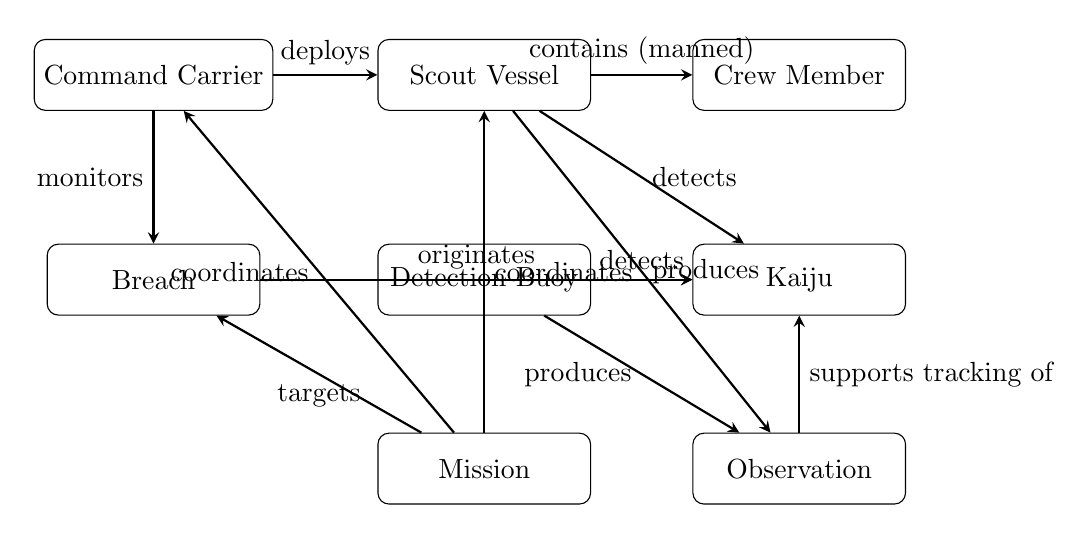
\begin{tikzpicture}[
        entity/.style={draw, rectangle, rounded corners, align=center, minimum width=2.7cm, minimum height=0.9cm},
        rel/.style={->, >=stealth, thick}
    ]
        \node[entity] (carrier) at (0, 2.2) {Command Carrier};
        \node[entity] (scout) at (4.2, 2.2) {Scout Vessel};
        \node[entity] (crew) at (8.2, 2.2) {Crew Member};
        \node[entity] (buoy) at (4.2, -0.4) {Detection Buoy};
        \node[entity] (kaiju) at (8.2, -0.4) {Kaiju};
        \node[entity] (breach) at (0, -0.4) {Breach};
        \node[entity] (mission) at (4.2, -2.8) {Mission};
        \node[entity] (observation) at (8.2, -2.8) {Observation};

        \draw[rel] (carrier) -- node[above] {deploys} (scout);
        \draw[rel] (scout) -- node[above] {contains (manned)} (crew);
        \draw[rel] (carrier) -- node[left] {monitors} (breach);
        \draw[rel] (breach) -- node[above] {originates} (kaiju);
        \draw[rel] (scout) -- node[right] {detects} (kaiju);
        \draw[rel] (buoy) -- node[above] {detects} (kaiju);
        \draw[rel] (mission) -- node[left] {coordinates} (carrier);
        \draw[rel] (mission) -- node[right] {coordinates} (scout);
        \draw[rel] (mission) -- node[below] {targets} (breach);
        \draw[rel] (scout) -- node[right] {produces} (observation);
        \draw[rel] (buoy) -- node[left] {produces} (observation);
        \draw[rel] (observation) -- node[right] {supports tracking of} (kaiju);
    \end{tikzpicture}
    \caption{High-level domain model for the Abyssal Watch case study.}
    \label{fig:case_study_domain_model}
\end{figure}

The figure in \autoref{fig:case_study_domain_model} is deliberately conceptual: it captures the principal entities and operational relationships, but omits attributes and storage concerns. This level of detail is enough to establish a shared mental model for the rest of the book. \todo{fix the diagram, what even is this}
